\documentclass[11pt]{article}
\usepackage[margin=1in]{geometry}
\usepackage{booktabs,longtable,array,graphicx,enumitem}
\usepackage[hidelinks]{hyperref}
\setlength{\parindent}{0pt}
\setlength{\parskip}{6pt}
\renewcommand{\arraystretch}{1.15}
\newcommand{\plainbox}[1]{\par\vspace{2pt}\noindent\fbox{\parbox{\dimexpr\linewidth-2\fboxsep-2\fboxrule\relax}{#1}}\par\vspace{2pt}}
\begin{document}
{\Large\textbf{Tasks Module, Part 4: The Ropeway Analysis}}\par
{\large Which workers could take the jobs the ropeway may bring, and how many may be left without work}\par\vspace{4pt}\hrule\vspace{8pt}

\plainbox{\textbf{Remember.} The workers are \textbf{made-up}. The number of ropeway jobs is a \textbf{placeholder} (we do not know it yet).
The job task lists are \textbf{provisional}, taken from the national occupation list. The results show how the method works and what it can and cannot say.
They are not a forecast.}

\section*{1. The question}
If the ropeway takes work away from people who carry pilgrims and goods on the trek, how many of them might end up without work?
Two things decide this. First, \emph{how many new jobs there are}. Second, \emph{whether the people who lose work can actually do those jobs}.
The task questions help with the second thing.

\section*{2. Which jobs might people move to?}
We listed 13 jobs that a ropeway and the trade around it may bring. Each has a short list of tasks it needs.
The lists come from the national occupation list (NCO 2015), so we can say where each one comes from. Where the list does not cover a job, we used judgement and say so.
Some jobs also need a paper (a licence or certificate). We call that a \textbf{gate}: without it the person cannot take the job, however many tasks they know.
{\scriptsize
\begin{longtable}{p{0.9cm}p{2.8cm}p{3.8cm}p{3.6cm}p{2.9cm}}
\toprule
\textbf{Id} & \textbf{Job} & \textbf{Tasks it needs} & \textbf{Where from} & \textbf{Gate} \\
\midrule
\endfirsthead
\toprule
\textbf{Id} & \textbf{Job} & \textbf{Tasks it needs} & \textbf{Where from} & \textbf{Gate} \\
\midrule
\endhead
RW1 & Aerial ropeway operator & 8 operate an engine or machine; 12 check equipment for safety; 24 coordinate by phone, radio, signals & NCO 8343.1700 & none \\
RW2 & Electrician / wireman (ropeway plant) & 10 electrical or wiring work; 12 check equipment for safety & NCO 7411.0301 (QP ELE/Q7302, NSQF 3) & ITI or NSQF-3 electrical certificate \\
RW3 & Mechanic / fitter (ropeway plant) & 8 operate an engine or machine; 9 repair by hand & NCO 7231.0500 (nearest entry) & ITI or technical certificate (assumed) \\
RW4 & Station loading and crowd attendant & 3 load, unload, stack, count goods; 23 keep order or watch property; 24 coordinate by phone, radio, signals & NCO 9333 loader + 8343.1700 attendant; judgement & none \\
RW5 & Ticket and information counter clerk & 16 handle cash and payments; 25 keep records or accounts; 21 guide or explain to visitors & NCO 4224.0100 / 4221 (nearest); judgement & none \\
SEC & Security guard / gateman & 23 keep order or watch property; 21 guide or explain to visitors; 25 keep records or accounts & NCO 5414 Gateman/Unarmed Security Guard (QP SKS/Q0101, NSQF 4) & NSQF-4 guard certificate \\
HOS1 & Room attendant / housekeeping & 20 clean rooms or public areas & NCO 5151.0202 & none \\
HOS2 & Waiter / food and beverage steward & 19 serve guests; 16 handle cash and payments & NCO 5131.0401 (NSQF 3, training-linked) & none \\
HOS3 & Cook & 18 cook or prepare food or drink & NCO 5120.0300 / 5122 & none \\
TRA & Light motor vehicle (car) driver & 7 drive a motor vehicle; 12 check equipment for safety; 16 handle cash and payments & NCO 8322.0100 & Car (LMV) licence \\
SHP & Shop assistant & 14 sell goods or services; 4 pack or tie goods & NCO 5223.0200 & none \\
GDE & Tourist guide & 21 guide or explain to visitors & NCO 5113.0200 & Guide or trekking permit (assumed; not in NCO) \\
CON & Construction labourer (build phase) & 11 build or construct; 1 carry loads on foot; 3 load, unload, stack, count goods & NCO 9313.9900 & none \\
\bottomrule
\end{longtable}
}

\textbf{Two cautions.} (1) The national list gives only 1 to 3 tasks for most of these jobs. That is few (see section 6). (2) The gate for ropeway operator, mechanic and guide is our assumption, since the national list does not state one.
Before real use, these lists should be checked with the ropeway company, hotel owners and unions.

\section*{3. Two simple measures}
For each worker and each job we count:
\begin{itemize}[leftmargin=1.2em,itemsep=2pt]
\item \textbf{Shortage}: of the tasks the new job needs, what share does the worker \emph{not} do? 0 means they can do all of them. 1 means none.
\item \textbf{Unused}: of the tasks the worker does now, what share would the new job not use? High means a lot of their skill goes to waste.
\end{itemize}
(These two ideas come from Neffke and co-authors, 2024, but their version uses many skills per job; ours uses tasks that are answered yes or no.)
We use two views of what a worker can do. \textbf{Strict}: only tasks done regularly now. \textbf{Broad}: tasks done regularly plus tasks done before (answer 2).

\textbf{Rule fixed before looking at the data:} a worker \emph{could take} a job if the shortage is one-third or less, \emph{and} the worker holds any gate paper. The base case uses the broad view.
We also test other cut-offs (0 and one-half).

\textbf{Worked example.} Worker 106 is a palki. The job ``construction labourer (build phase)'' needs: 11 build or construct; 1 carry loads on foot; 3 load, unload, stack, count goods.
Doing tasks regularly now, the worker lacks 2 of the 3 (shortage 0.67), so the strict view says \emph{no}.
The worker also did before: 3 load, unload, stack, count goods. In the broad view the shortage is 0.33 and the answer is \emph{yes}.
This is the reason we ask answer 2 on the task grid.

\section*{4. Who is exposed to the ropeway?}
We need to know whose work the ropeway may replace. The test data gives three ways to decide:
{\small
\begin{longtable}{p{11cm}r}
\toprule
\textbf{Way of deciding} & \textbf{Workers} \\
\midrule
\endfirsthead
\toprule
\textbf{Way of deciding} & \textbf{Workers} \\
\midrule
\endhead
By job title: porters, palki bearers, pony workers, pony owners & 26 \\
By main task: carrying, passenger, or pack animals & 23 \\
By any regular carrying, passenger or pack-animal task & 66 \\
\bottomrule
\end{longtable}
}

The first is used in the base case (26 workers). The second misses pony people whose main task is feeding animals, loading, or selling rides, and it includes one wage labourer.
The third counts 66 workers, including many shop and hotel workers who sometimes carry loads. This is too wide.
\textbf{Lesson.} Exposure should not be guessed from a task or a title. The survey needs its own direct exposure questions (module D), such as ``does your income come from taking people or goods on the Kedarnath trek?''.

\section*{5. Who could take which job?}
The picture and table show, for the 26 exposed workers, the share who pass the rule for each job.
\begin{center}
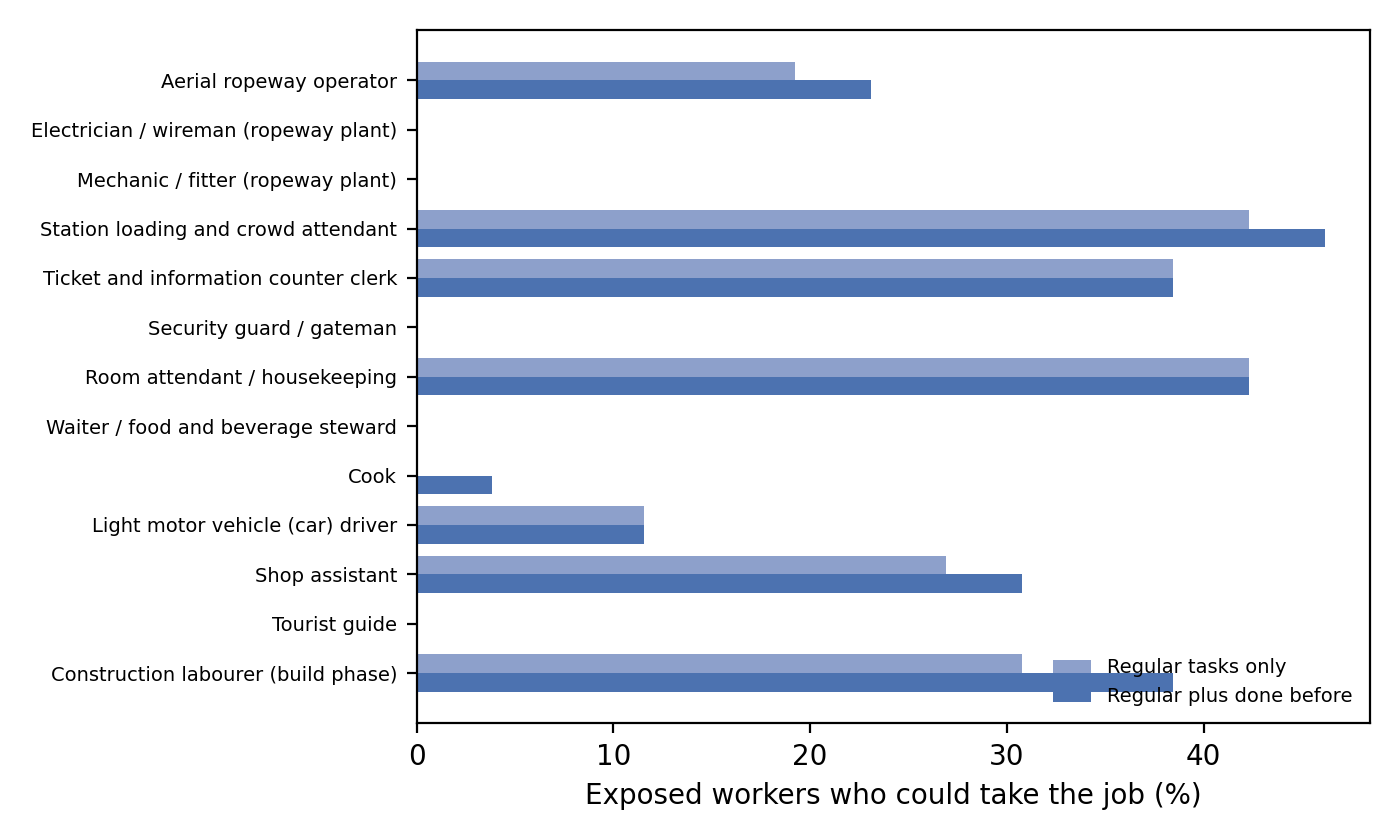
\includegraphics[width=0.85\linewidth]{../03_analysis/outputs/4_5_eligible.png}\\[2pt]
{\small Share of exposed workers who could take each job (shortage one-third or less, and gate paper held).}
\end{center}
{\footnotesize
\begin{longtable}{p{5.2cm}rrrrr}
\toprule
\textbf{Job} & \textbf{Tasks} & \textbf{Hold gate, all workers (\%)} & \textbf{Strict (\%)} & \textbf{Broad (\%)} & \textbf{Broad, no gate (\%)} \\
\midrule
\endfirsthead
\toprule
\textbf{Job} & \textbf{Tasks} & \textbf{Hold gate, all workers (\%)} & \textbf{Strict (\%)} & \textbf{Broad (\%)} & \textbf{Broad, no gate (\%)} \\
\midrule
\endhead
Aerial ropeway operator & 3 & 100 & 19 & 23 & 23 \\
Electrician / wireman (ropeway plant) & 2 & 10 & 0 & 0 & 8 \\
Mechanic / fitter (ropeway plant) & 2 & 10 & 0 & 0 & 0 \\
Station loading and crowd attendant & 3 & 100 & 42 & 46 & 46 \\
Ticket and information counter clerk & 3 & 100 & 38 & 38 & 38 \\
Security guard / gateman & 3 & 3 & 0 & 0 & 31 \\
Room attendant / housekeeping & 1 & 100 & 42 & 42 & 42 \\
Waiter / food and beverage steward & 2 & 100 & 0 & 0 & 0 \\
Cook & 1 & 100 & 0 & 4 & 4 \\
Light motor vehicle (car) driver & 3 & 17 & 12 & 12 & 54 \\
Shop assistant & 2 & 100 & 27 & 31 & 31 \\
Tourist guide & 1 & 3 & 0 & 0 & 38 \\
Construction labourer (build phase) & 3 & 100 & 31 & 38 & 38 \\
\bottomrule
\end{longtable}
}

\begin{itemize}[leftmargin=1.2em,itemsep=2pt]
\item The jobs closest to carrying work (station attendant, room attendant, construction, ticket counter) suit 38--46 in 100 exposed workers.
\item The technical ropeway jobs (electrician, mechanic) suit almost no one. Few people hold an ITI or similar paper, and fewer do electrical or engine work.
\item Guard, guide and driver jobs are open on tasks to many, but few hold the paper. \textbf{Gates matter more than tasks for these jobs.} This is why the questions on licences (T3) are in the survey.
\item On average an exposed worker could take \textbf{2.3} of the 13 jobs.
\textbf{15 in 100} could take none at all (19 in 100 in the strict view). Weighted for drop-out, 16 in 100.
\end{itemize}
The number who could take \emph{no} job is important. It does not depend on how many jobs exist. It is a floor: even if jobs were unlimited, these workers could not be placed with the tasks and papers they hold now.

\section*{6. Type of move, and a warning}
Neffke and co-authors sort moves into four types by combining shortage and unused skills: a \emph{close match} (low, low), \emph{downskilling} (few tasks to add, many unused), \emph{upskilling} (many to add, few unused), and \emph{reskilling} (many to add, many unused).
{\small
\begin{longtable}{lrr}
\toprule
\textbf{Type of move} & \textbf{All worker-job pairs (\%)} & \textbf{To the worker's closest job (\%)} \\
\midrule
\endfirsthead
\toprule
\textbf{Type of move} & \textbf{All worker-job pairs (\%)} & \textbf{To the worker's closest job (\%)} \\
\midrule
\endhead
close match & 1 & 0 \\
downskill (surplus skills) & 27 & 88 \\
upskill (tasks to add) & 0 & 0 \\
reskill (start over) & 73 & 12 \\
\bottomrule
\end{longtable}
}
\begin{center}
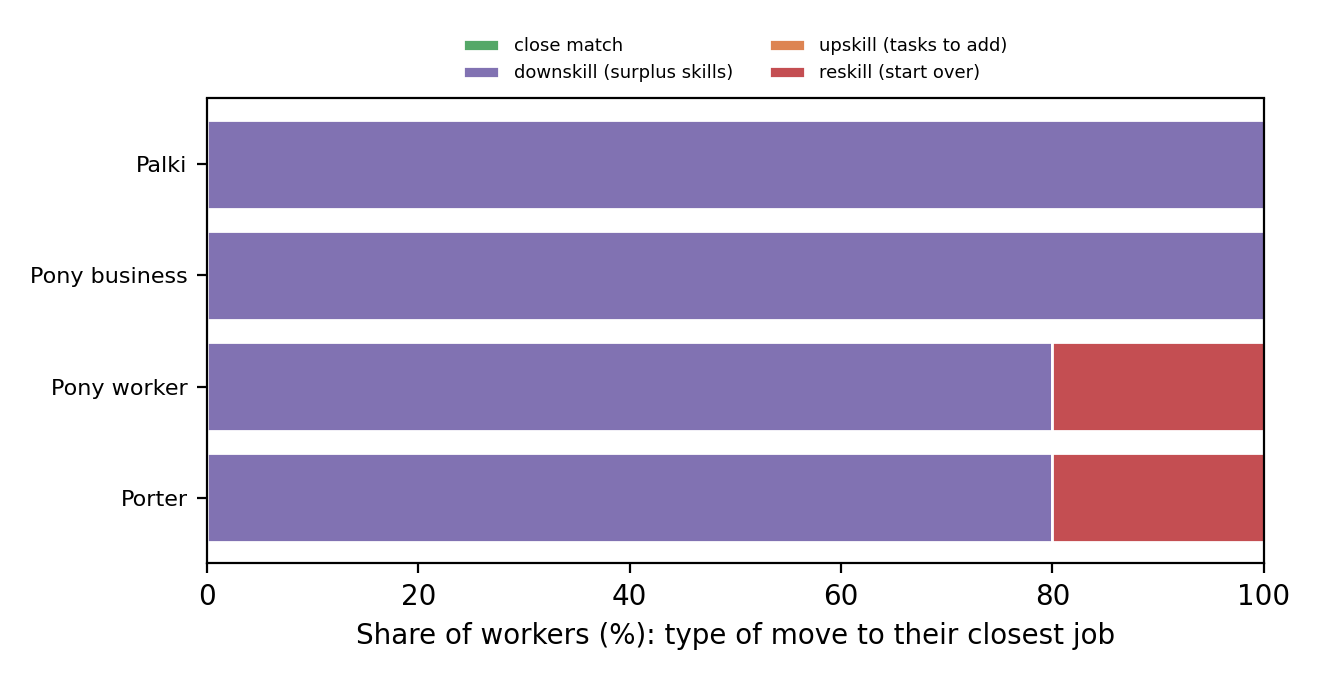
\includegraphics[width=0.7\linewidth]{../03_analysis/outputs/4_3_types.png}\\[2pt]
{\small Type of move to each worker's closest job, by present job.}
\end{center}

Almost every move is called ``downskilling'' or ``reskilling'', and 99 in 100 pairs have a high ``unused'' share.
This is not a finding. It happens because our job lists have only about 2.2 tasks while a worker does about 7.4, so most of what the worker does can never be used by a short list.
\textbf{Lesson.} The ``unused'' measure and the four types need long task lists for each job (10 or more). With the short lists we have, use \textbf{shortage only}. To use the four types, the survey needs job task lists from employers or a ropeway operator.

We also checked whether the closest job changes with the measure. The closest job by shortage is the same as the closest by two other common measures (cosine and Jaccard) for 62 in 100 workers.
So the ranking of jobs \emph{is} sensitive to the measure when job lists are short. Shortage is the only measure with a plain meaning (``how many of the new job's tasks are new to me''), so we keep it.

\section*{7. How many may be left without work?}
We count three things, all per 100 exposed workers:
\begin{itemize}[leftmargin=1.2em,itemsep=2pt]
\item \textbf{Numbers only}: exposed workers minus new jobs. This is what most reports do. It ignores who can do what.
\item \textbf{Skills, best possible}: give jobs to workers so that as many as possible are placed, each worker only in a job they could take (maximum matching). This is the best case.
\item \textbf{Skills, by lottery}: jobs are given at random among workers who could take them, repeated 300 times. This is closer to how hiring might go.
\end{itemize}
\textbf{Job supply is a placeholder.} We tried three totals (25, 50 and 100 new jobs per 100 exposed workers) and three mixes (equal across job types; three times as many technical jobs; three times as many service jobs). The real numbers must come from the ropeway plan and an employer check.
\begin{center}
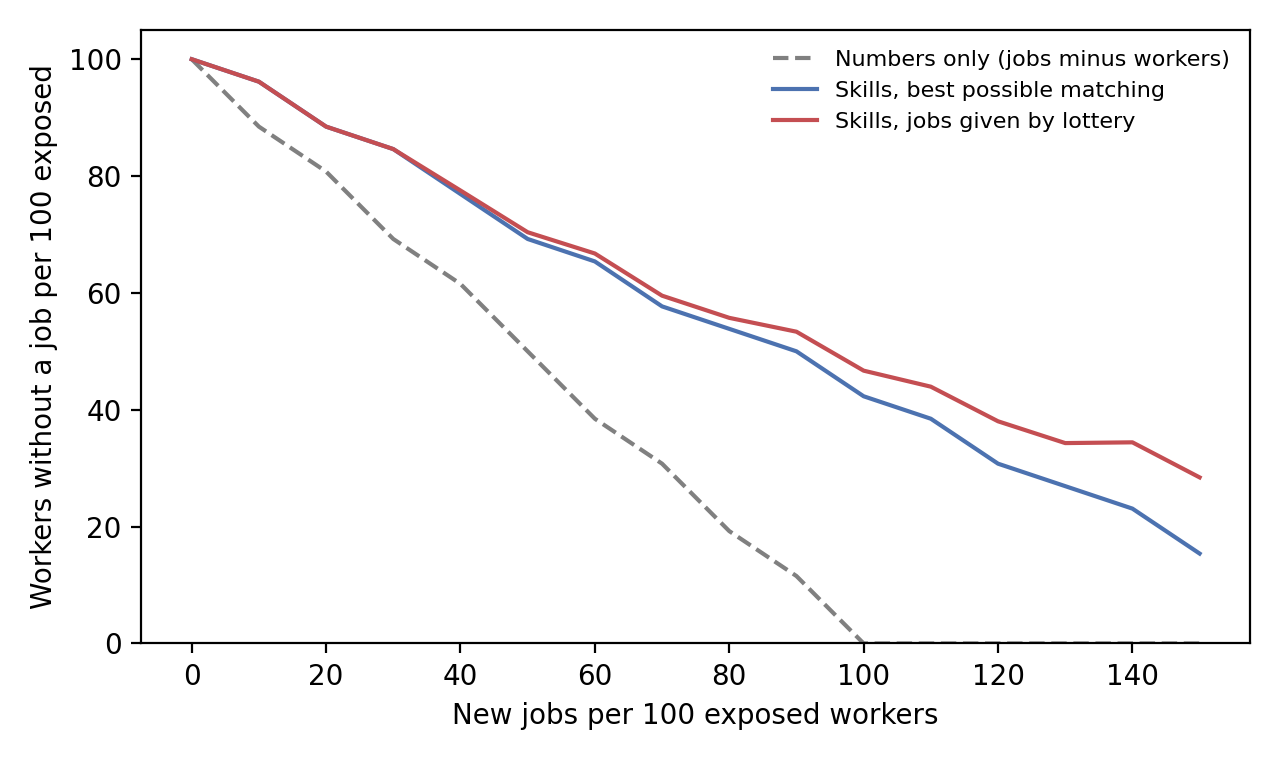
\includegraphics[width=0.7\linewidth]{../03_analysis/outputs/4_6_curve.png}\\[2pt]
{\small Workers left without a job per 100 exposed, as new jobs increase (equal mix).}
\end{center}
{\small
\begin{longtable}{rlrrr}
\toprule
\textbf{New jobs per 100 exposed} & \textbf{Mix} & \textbf{Numbers only} & \textbf{Skills, best} & \textbf{Skills, lottery} \\
\midrule
\endfirsthead
\toprule
\textbf{New jobs per 100 exposed} & \textbf{Mix} & \textbf{Numbers only} & \textbf{Skills, best} & \textbf{Skills, lottery} \\
\midrule
\endhead
25 & equal & 77 & 88 & 88 \\
25 & technical-heavy & 77 & 88 & 88 \\
25 & service-heavy & 77 & 85 & 85 \\
50 & equal & 50 & 69 & 70 \\
50 & technical-heavy & 50 & 73 & 73 \\
50 & service-heavy & 50 & 73 & 74 \\
100 & equal & 0 & 42 & 47 \\
100 & technical-heavy & 0 & 46 & 51 \\
100 & service-heavy & 0 & 42 & 45 \\
\bottomrule
\end{longtable}
}

\textbf{Reading the table.} In the middle case (50 new jobs per 100 exposed, equal mix), numbers alone give 50 without a job per 100.
Once tasks and papers are taken into account, it is \textbf{69} in the best case and \textbf{71} by lottery.
Resampling the workers 1{,}000 times gives a range of about 69 to 73 for the best case. That range comes only from having few workers; it does not include uncertainty about the job supply or the job lists, which are larger.

Even if there were \textbf{one new job for every exposed worker}, about 42 in 100 would still be without work, because the new jobs are of the wrong kind or need papers.
When there are more technical jobs, the number without work is higher.

\section*{8. Do the choices change the answer?}
The middle case (50 new jobs per 100 exposed, equal mix, exposed by job title) under different rules:
{\footnotesize
\begin{longtable}{llrrrr}
\toprule
\textbf{View} & \textbf{Shortage cut} & \textbf{Gates} & \textbf{Could take no job (\%)} & \textbf{Numbers only} & \textbf{Skills, best} \\
\midrule
\endfirsthead
\toprule
\textbf{View} & \textbf{Shortage cut} & \textbf{Gates} & \textbf{Could take no job (\%)} & \textbf{Numbers only} & \textbf{Skills, best} \\
\midrule
\endhead
strict & 0.00 & yes & 42 & 50 & 85 \\
strict & 0.00 & no & 19 & 50 & 73 \\
strict & 0.30 & yes & 19 & 50 & 73 \\
strict & 0.30 & no & 15 & 50 & 62 \\
strict & 0.50 & yes & 4 & 50 & 69 \\
strict & 0.50 & no & 4 & 50 & 54 \\
broad & 0.00 & yes & 38 & 50 & 77 \\
broad & 0.00 & no & 19 & 50 & 65 \\
broad & 0.30 & yes & 15 & 50 & 69 \\
broad & 0.30 & no & 12 & 50 & 58 \\
broad & 0.50 & yes & 0 & 50 & 65 \\
broad & 0.50 & no & 0 & 50 & 50 \\
\bottomrule
\end{longtable}
}

\begin{itemize}[leftmargin=1.2em,itemsep=2pt]
\item A stricter rule (cut 0) or the strict view raises the count. A looser rule (cut one-half) lowers it. \textbf{The result is quite sensitive to the cut}, so real results should show all three.
\item Ignoring gates lowers the count by about 10 points. Gates matter.
\item If we require the optional tasks too, the share who could take no job rises to 35 in 100.
\item If the ropeway operator job needs a certificate, the answer barely changes here.
\item Using the other two ways of deciding who is exposed:
\end{itemize}

\section*{9. What we learn for the survey}
\begin{enumerate}[leftmargin=1.4em,itemsep=2pt]
\item \textbf{Keep the three-answer task grid.} Answer 2 changes who could take a job, though not by a lot.
\item \textbf{Keep the licence and certificate questions (T3).} Gates decide more than tasks for the driver, guard, guide and technical jobs.
\item \textbf{Add direct exposure questions (module D).} Exposure cannot be guessed from job titles or tasks.
\item \textbf{Get long task lists for the destination jobs.} The national list is too short for the ``unused'' measure. A short employer or operator questionnaire can give this, and also the number of jobs.
\item \textbf{Report ranges, not one number.} The result depends on the cut, the gate rules, the job supply and the job mix.
\item \textbf{More workers in the small groups.} Twenty-six exposed workers give crude results. The real quota should give enough in each of the four exposed jobs.
\end{enumerate}

\section*{10. What this cannot tell us}
\begin{itemize}[leftmargin=1.2em,itemsep=2pt]
\item The job supply is invented. The answer is a function of it.
\item Only exposed workers compete for jobs here. In fact others (workers from elsewhere, other locals) will also apply, so real competition is stronger and the count without work is a \textbf{lower} figure.
\item Workers may also lose part of their work rather than all of it, or move into work that is not on the list (for example their own small business). We do not count that here.
\item Having the tasks is not the same as being hired. Age, health, language, caste and contacts also matter and are not in this analysis.
\item The task answers were made from our own rules, so agreement with them is not evidence about the world.
\end{itemize}

\section*{11. Files}
\begin{itemize}[leftmargin=1.2em,itemsep=1pt]
\item \texttt{03\_analysis/specific\_analysis.py}: the code. \texttt{03\_analysis/results\_specific.json}: all numbers.
\item \texttt{03\_analysis/outputs/4\_1} to \texttt{4\_7}: tables and pictures. The destination job list is \texttt{4\_1\_destination\_jobs.csv}.
\end{itemize}
\end{document}
